\chapter{Graph-Datenbanken im praktischen Einsatz: OLAP}
\section{PostgreSQL: OLAP}
\subsection{Benchmark}
Mit der Standardinstallation von PostgreSQL wird auch pgbench mitinstalliert. Bei pgbench handelt es sich um ein einfaches Tool zur Durchführung von Benchmark-Tests. Bei einem Benchmark-Test wird eine Menge von \ac{SQL}-Statements beliebig oft wiederholt, dabei können auch mehrere parallele Sessions geöffnet werden. Beim durchführen des Tests berechnet pgbench die Anzahl der Transaktionen pro Sekunde.
\subsubsection{Verwendung von pgbench}
pgbench wird über die Kommandozeile gestartet. Dabei können eine Reihe von Parametern übergeben werden, mit denen das Verhalten von pgbench gesteuert werden kann.
\begin{itemize}
	\item -c clients  \\
	Über das Flag -c wird die Anzahl der Clients bzw. die Anzahl der gleichzeitigen Datenbankverbindungen festgelegt. Wenn hier nichts angegeben ist wird nur ein Client verewendet.
	\item -t transactions \\
	Über das Flag -t wird festgelegt wieviele Transaktionen jeder Client durchführt. Die Anzahl aller Transaktionen ergibt sich durch das Produkt von Clients und Transactions.
\end{itemize}
\subsubsection{selectSourceCodeGenerator}
\begin{figure}[H]
\begin{tikzpicture}[y=.01cm, x=2cm,font=\sffamily]
%axis
\draw (0,0) -- coordinate (x axis mid) (5,0);
\draw (0,0) -- coordinate (y axis mid) (0,700);
    	%ticks
\foreach \x in {0,...,5}
\draw (\x,1pt) -- (\x,-3pt)
node[anchor=north] {\x};
\foreach \y in {0,50,...,700}
\draw (1pt,\y) -- (-3pt,\y)
node[anchor=east] {\y}; 
%labels      
\node[below=0.8cm] at (x axis mid) {Rekursionstiefe};
\node[rotate=90, above=1.5cm] at (y axis mid) {Laufzeit in ms};
%plots
\draw plot[mark=*, mark options={fill=white}] 
coordinates{(0, 0)
			(1, 63.636)
			(2,139.225)
			(3,229.997)
			(4,432.297)
			(5,677.420)
		};
\end{tikzpicture}
	\caption{ public\_epinions}
\end{figure}


\begin{table}[H]
	\centering
	\begin{tabular}{|l|l|}
		\hline
		Rerkusionstiefe & Laufzeit in ms \\ \hline
		1               & 63.636         \\ \hline
		2               & 139.225        \\ \hline
		3               & 229.997        \\ \hline
		4               & 432.297        \\ \hline
		5               & 677.420        \\ \hline
	\end{tabular}
\end{table}

\begin{figure}[H]
	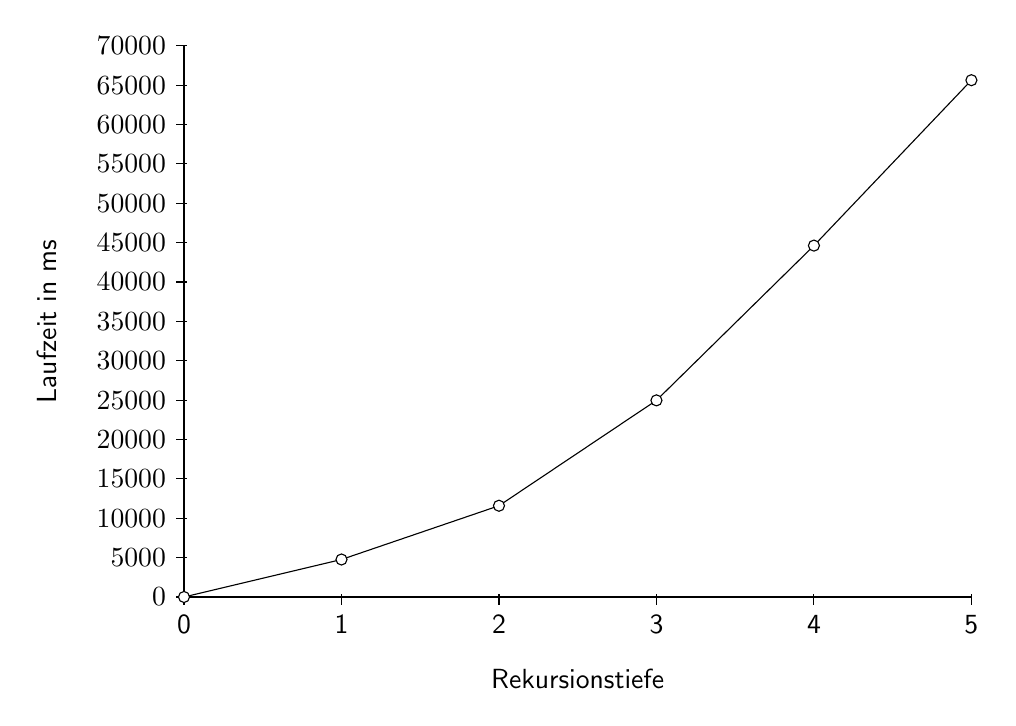
\begin{tikzpicture}[y=.5cm, x=2cm,font=\sffamily]
	%axis
	\draw (0,0) -- coordinate (x axis mid) (5,0);
	\draw (0,0) -- coordinate (y axis mid) (0,14);
	%ticks
	\foreach \x in {0,...,5}
	\draw (\x,1pt) -- (\x,-3pt)
	node[anchor=north] {\x};
	\foreach \y/\ytext in {
		0/0,
		1/5000,
		2/10000,
		3/15000,
		4/20000,
		5/25000,
		6/30000,
		7/35000,
		8/40000,
		9/45000,
		10/50000,
		11/55000,
		12/60000,
		13/65000,
		14/70000
	}
	\draw (1pt,\y) -- (-3pt,\y) node[anchor=east] {$\ytext$};
	%labels      
	\node[below=0.8cm] at (x axis mid) {Rekursionstiefe};
	\node[rotate=90, above=1.5cm] at (y axis mid) {Laufzeit in ms};
	%plots
	\draw plot[mark=*, mark options={fill=white}] 
	coordinates{(0, 0)
		(1, 4761.733/5000)
		(2,	11589.219/5000)
		(3, 4.9944)	%=24971/5000
		(4, 8.9252) %=44625,935÷5000
		(5,	13.1265944)%=65632,972÷5000
	};
	\end{tikzpicture}
	\caption{ public\_livejournal}
\end{figure}
\subsection{Standard SQL}
\subsection{Stored Procedures}
\subsection{PL/SQL-Recursion}
\subsection{Datenbankzugriffe}
\subsection{Zugriffsart Aggregation}
\subsection{Zugriffsart Traversierung}
\subsection{Interpretation der Ergebnisse}